\documentclass[a4paper,12pt]{article}

\usepackage[utf8]{inputenc}
\usepackage[T1]{fontenc}
\usepackage[polish]{babel}
\usepackage{amsmath, amssymb}
\usepackage{graphicx}
\usepackage{float}
\usepackage{hyperref}
\usepackage{geometry}
\usepackage{csvsimple} 

\geometry{margin=2.5cm}

\title{Sprawozdanie 1 z Statystyki i Modeli Liniowych}
\author{Wiktor Zoga}
\date{\today}

\begin{document}

\maketitle
\newpage

\section{Zadanie 1}

\subsection{Opis eksperymentu}
W tym zadaniu wygenerowano $n$ obserwacji z rozkładu normalnego $N(\theta, \sigma^2)$ dla następujących zestawów parametrów:

\begin{enumerate}
    \item $\theta = 0$, $\sigma = 1$
    \item $\theta = 0$, $\sigma = 2$
    \item $\theta = 4$, $\sigma = 1$
    \item $\theta = 4$, $\sigma = 2$
\end{enumerate}

Dla każdej próbki obliczono siedem estymatorów wartości oczekiwanej:

\begin{itemize}
    \item $\hat{\theta}_1$ -- średnia arytmetyczna
    \item $\hat{\theta}_2$ -- mediana
    \item $\hat{\theta}_3$ -- ważona średnia z własnymi wagami
    \item $\hat{\theta}_4$ -- estymator z wagami zależnymi od dystrybuanty normalnej
    \item $\hat{\theta}_5$ -- średnia harmoniczna
    \item $\hat{\theta}_6$ -- średnia potęgowa rzędu 3
    \item $\hat{\theta}_7$ -- własny estymator (średnia z minimum i maksimum próby)
\end{itemize}

Doświadczenie powtórzono $10{,}000$ razy dla każdego zestawu parametrów i rozmiarów próbek $n = 20, 50, 100$.

\newpage

\subsection{Wyniki - wykresy pudełkowe i tabele statystyk}

\newcommand{\offplotwithstats}[3]{
    \begin{figure}[H]
        \centering
        \includegraphics[width=0.9\textwidth]{../Zad1/plots/5_off_boxplot_theta#1_sigma#2_n#3.png}
        \caption{Boxplot estymatorów bez piątego.}
    \end{figure}
}

\newcommand{\plotwithstats}[3]{
    \subsection{$\theta=#1$, $\sigma=#2$, $n=#3$}
    \begin{figure}[H]
        \centering
        \includegraphics[width=0.9\textwidth]{../Zad1/plots/boxplot_theta#1_sigma#2_n#3.png}
        \caption{Boxplot estymatorów dla $\theta=#1$, $\sigma=#2$, $n=#3$.}
    \end{figure}

    \offplotwithstats{#1}{#2}{#3}

    \begin{center}
    \csvreader[
        tabular=|l|c|c|c|c|,
        table head=\hline Estymator & Średnia & Wariancja & Bias & MSE \\ \hline,
        late after line=\\\hline,
        filter expr={true},  % brak filtrowania
        respect percent
    ]{../Zad1/plots/stats_theta#1_sigma#2_n#3.csv}{Estimator=\est,Mean=\mean,Variance=\var,Bias=\bias,MSE=\mse}
    {\est & \pgfmathprintnumber{\mean} & \pgfmathprintnumber{\var} & \pgfmathprintnumber{\bias} & \pgfmathprintnumber{\mse} }
    \end{center}

    % \newpage
}

\plotwithstats{0}{1}{20}
\plotwithstats{0}{1}{50}
\plotwithstats{0}{1}{100}

\plotwithstats{0}{2}{20}
\plotwithstats{0}{2}{50}
\plotwithstats{0}{2}{100}

\plotwithstats{4}{1}{20}
\plotwithstats{4}{1}{50}
\plotwithstats{4}{1}{100}

\plotwithstats{4}{2}{20}
\plotwithstats{4}{2}{50}
\plotwithstats{4}{2}{100}

\subsection{Dyskusja Wyników}

\subsubsection{Est1 - Średnia Arytmetyczna}
Zgodnie z teorią estymacji, średnia arytmetyczna jest nieobciążonym estymatorem średniej w rozkładzie normalnym.
Wyniki symulacji to potwierdzają – $\hat{\theta}_1$ wykazuje obciążenie bliskie zeru 
oraz najniższą wariancję (i tym samym najniższe MSE) spośród wszystkich badanych estymatorów nieobciążonych. 
Służy jako dobry punkt odniesienia.

\subsubsection{Est2 - Mediana}
Mediana również jest estymatorem nieobciążonym dla rozkładu normalnego. 
Wynika to z tego, że rozkład ma symetryczną gęstość, a mediana ma "własność przesunięcia".
Jej wariancja jest jednak wyższa niż wariancja średniej arytmetycznej,
co potwierdzają wyniki MSE. 
Dla średniej rozkładu normalnego, jest to estymator mniej efektywny niż średnia arytmetyczna, 
choć bardziej odporny na wartości odstające (co nie było przedmiotem tego badania).

\subsubsection{Est3 - Ważona Średnia}
Ważona średnia (losowe wagi o sumie jeden) jest estymatorem nieobciążonym, który może być bardziej efektywny niż średnia arytmetyczna w przypadku rozkładów o asymetrycznych ogonach.
W przypadkach rozkładu normalnego, nie gra to większej roli, a MSE jest lekko wyższy niż dla średniej arytmetycznej.

\subsubsection{Est4 - Ważona Średnia wagami z Dystrybuanty Normalnej}
Ten estymator jest obciążony ponieważ wagi nie sumują się do 1. Po mimo zauważalnie mniejszej wariancji 
od innych estymatorów ma duży bias co przekłada się na wysokie MSE.

\subsubsection{Est5 - Średnia Harmoniczna}
Średnia harmoniczna jest estymatorem obciążonym, szczególnie w przypadku rozkładów z dużą wariancją.
Wyniki pokazują znaczne obciążenie i wysokie MSE, co czyni ją nieodpowiednią do estymacji średniej w rozkładzie normalnym.
Wynika to głównie z faktu, że $\frac{1}{X}$ nie jest funkcją całkowaną z gestością rozkładu normalnego.

\subsubsection{Est6 - Średnia Potęgowa Rzędu 3}
Dzięki mocnemu prawu wielkich liczb średnia potęgowa rzędu 3 jest estymatorem asymptotycznie nieobciążonym, ale jedynie dla średniej 0.
W przypadkach z $\theta = 4$ jest zauważalny bias.
Wariancja jest jednak wyższa niż w przypadku średniej arytmetycznej, co czyni ją mniej efektywną w praktyce.

\subsubsection{Est7 - Średnia z Minimum i Maksimum Próby}
Ten estymator jest nieobciążony, co wynika z bezpośredniej symetrii rozkładu normalnego (pomijam rachunki, ale wykonałem je).
Jednakże jego wariancja jest znacznie wyższa niż w przypadku innych estymatorów, gdyż nie maleje wraz ze wzrostem $n$ jak w przypadku innych estymatorów.
Teoretyczne wyliczenia wariancji nie są już tak proste, jednak wyniki symulacji pokazują, że jest ona wyższa niż w przypadku średniej, ale wciąż nie duża.

\section{Zadanie 2}

\subsection{Opis eksperymentu}
W tym zadaniu dla kolejnych parametrów

\begin{enumerate}
    \item $\theta = 0$, $\sigma = 1$
    \item $\theta = 0$, $\sigma = 2$
    \item $\theta = 4$, $\sigma = 1$
    \item $\theta = 4$, $\sigma = 2$
\end{enumerate}

wygenerowano próby o rozmiarze $n=50$ z rozkładów: $ N(\theta, \sigma^2), Logist(\theta, \sigma), Cauchy(\theta, \sigma)$.

Dla każdej próbki obliczono dwa estymatory:

\begin{itemize}
    \item $\hat{\theta}_1$ -- średnia arytmetyczna
    \item $\hat{\theta}_2$ -- mediana
\end{itemize}

Doświadczenie powtórzono $10{,}000$ razy dla każdego zestawu parametrów i rozkładu.

\newpage

\subsection{Wyniki - wykresy pudełkowe i tabele statystyk}

\newcommand{\plotwithstatsII}[3]{
    \subsection{$\theta=#1$, $\sigma=#2$}
    \begin{figure}[H]
        \centering
        \includegraphics[width=0.9\textwidth]{../Zad2/plots/boxplot_all_theta#1_sigma#2.png}
        \caption{Boxplot wszystkich rozkładów i estymatorów}
    \end{figure}

    \begin{figure}[H]
        \centering
        \includegraphics[width=0.9\textwidth]{../Zad2/plots/boxplot_no_cauchy_theta#1_sigma#2.png}
        \caption{Boxplot bez rozkładu cauchy'ego}
    \end{figure}

    \begin{center}
        \csvreader[
            tabular=|l|c|c|c|c|,
            table head=\hline Estymator & Średnia & Wariancja & Bias & MSE \\ \hline,
            late after line=\\\hline,
            filter expr={true},  % brak filtrowania
            respect percent
        ]{../Zad2/plots/table_theta#1_sigma#2.csv}{Estimator=\est,Mean=\mean,Variance=\var,Bias=\bias,MSE=\mse}
    {\est & \pgfmathprintnumber{\mean} & \pgfmathprintnumber{\var} & \pgfmathprintnumber{\bias} & \pgfmathprintnumber{\mse} }
    \end{center}

    \newpage
}

\plotwithstatsII{0}{1}

\plotwithstatsII{0}{2}

\plotwithstatsII{4}{1}

\plotwithstatsII{4}{2}

\subsection{Dyskusja}

W zadaniu analizowane są trzy rozkłady prawdopodobieństwa, wszystkie należące do rodziny rozkładów symetrycznych,
ale o fundamentalnie różnych właściwościach (szczególnie dotyczących tzw. "grubości ogonów").

\begin{itemize}
    \item \textbf{Rozkład Normalny (Gaussa) $\mathcal{N}(\theta, \sigma^2)$}
    Jego funkcja gęstości prawdopodobieństwa (PDF) dana jest wzorem:
    \[ f(x; \theta, \sigma^2) = \frac{1}{\sigma\sqrt{2\pi}} \exp\left(-\frac{(x-\theta)^2}{2\sigma^2}\right) \]
    \begin{itemize}
        \item $\theta$: Parametr położenia. Jest to jednocześnie \textbf{wartość oczekiwana}, \textbf{mediana} oraz \textbf{dominanta} rozkładu. $E[X] = \theta$.
        \item $\sigma^2$: Parametr skali. Jest to \textbf{wariancja} rozkładu.
    \end{itemize}
    
    \item \textbf{Rozkład Logistyczny $\text{Logist}(\theta, \sigma)$}
    Rozkład symetryczny, podobny kształtem do normalnego, ale o "grubszych ogonach". Jego PDF to:
    \[ f(x; \theta, \sigma) = \frac{\exp\left(-\frac{x-\theta}{\sigma}\right)}{\sigma\left(1 + \exp\left(-\frac{x-\theta}{\sigma}\right)\right)^2} \]
    \begin{itemize}
        \item $\theta$: Parametr położenia. Podobnie jak w rozkładzie normalnym, jest to \textbf{wartość oczekiwana}, \textbf{mediana} i \textbf{dominanta}. $E[X] = \theta$.
        \item $\sigma$: Parametr skali. Nie jest to odchylenie standardowe. Wariancja tego rozkładu jest skończona i wynosi $\text{Var}(X) = \frac{\sigma^2 \pi^2}{3}$.
    \end{itemize}

    \item \textbf{Rozkład Cauchy'ego $\text{Cauchy}(\theta, \sigma)$}
    Rozkład symetryczny znany z posiadania ekstremalnie "grubych ogonów". Jego PDF:
    \[ f(x; \theta, \sigma) = \frac{1}{\pi\sigma \left(1 + \left(\frac{x-\theta}{\sigma}\right)^2\right)} \]
    \begin{itemize}
        \item $\theta$: Parametr położenia. Ze względu na symetrię rozkładu, $\theta$ jest jego \textbf{medianą} oraz \textbf{dominantą}.
        \item $\sigma$: Parametr skali.
        \item \textbf{Kluczowa uwaga:} Dla rozkładu Cauchy'ego \textbf{wartość oczekiwana oraz wariancja nie istnieją}. Całka $E[|X|]$ jest rozbieżna.
    \end{itemize}
\end{itemize}

Tak wyglądają gęstości prawdopodobieństwa tych rozkładów:

\begin{figure}[H]
    \centering
    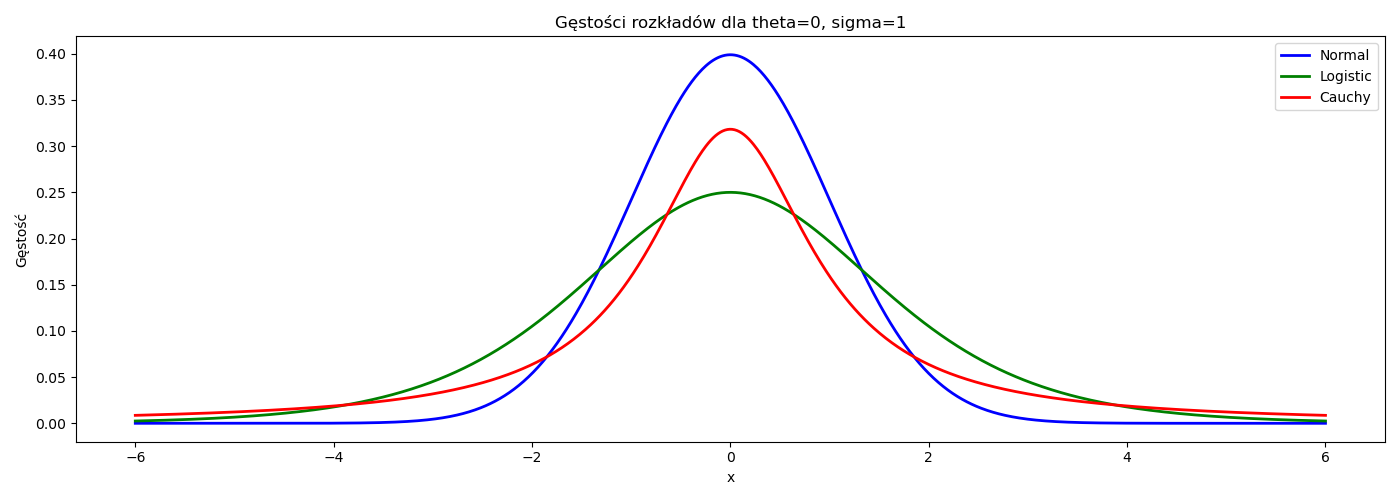
\includegraphics[width=1.0\textwidth]{../Zad2/plots/theoretical_density_theta0_sigma1.png}
    \caption{Funkcje gęstości prawdopodobieństwa rozkładów Normalnego, Logistycznego i Cauchy'ego dla $\theta=0$ i $\sigma=1$}
\end{figure}

\subsection{Dyskusja Wyników}

Analiza porównawcza estymatorów $\hat{\theta}_1$ (średnia arytmetyczna) i $\hat{\theta}_2$ (mediana) dla trzech różnych rozkładów symetrycznych ujawnia fundamentalne różnice we właściwościach tych estymatorów.

We wszystkich trzech badanych przypadkach parametr $\theta$ pełni rolę parametru położenia, definiując \textbf{oś symetrii} funkcji gęstości.

\subsection*{Analiza Estymatora $\hat{\theta}_1$ (Średnia Arytmetyczna)}

\begin{itemize}
    \item W przypadku rozkładu \textbf{Normalnego} oraz \textbf{Logistycznego}, wartość oczekiwana istnieje i jest równa osi symetrii, tzn. $E[X] = \theta$. Dlatego w tych dwóch przypadkach średnia arytmetyczna jest nieobciążonym estymatorem parametru $\theta$, co potwierdziły wyniki symulacji (bias niski, MSE niski).

    \item Rozkład \textbf{Cauchy'ego} jest jedynym spośród badanych, który jest \textbf{pozbawiony wartości oczekiwanej}. Jest to więc estymator całkowicie nieodpowiedni do estymacji parametru położenia tego rozkładu. Wyniki symulacji odzwierciedlają tę teoretyczną katastrofę, wykazując ekstremalnie wysoką wariancję i błąd MSE.
\end{itemize}

\subsection*{Analiza Estymatora $\hat{\theta}_2$ (Mediana)}

Dla \textit{każdego} rozkładu symetrycznego, oś symetrii $\theta$ \textbf{zawsze pokrywa się z medianą} rozkładu.

Mediana z próby ($\hat{\theta}_2$) jest estymatorem mediany populacji.

Wyniki symulacji potwierdzają tę tezę. Estymator $\hat{\theta}_2$ wykazał \textbf{dobre właściwości} (niskie obciążenie i niewielki błąd MSE) dla \textbf{wszystkich trzech rozkładów}. 
Ukazuje to jego \textbf{odporność} na ekstremalnie "grube ogony" rozkładu Cauchy'ego, dla którego średnia arytmetyczna zawiodła.

\section{Zadanie 3}

\subsection{Opis eksperymentu}
W tym zadaniu do próby wielkości $n-1=49$ z rozkładu $N(0, 1)$ dodano kolejne wartości $k=10, 20, ..., 100$

Na tej podstawie wyliczone dwa estymatory:

\begin{itemize}
    \item $\hat{\theta}_1$ -- średnia arytmetyczna
    \item $\hat{\theta}_2$ -- mediana
\end{itemize}

Doświadczenie powtórzono $10{,}000$ razy dla każdego zestawu z $k$. 
Błąd średniokwadratowy, obciążenie i wariancja zostały przedstawione na wykresie w zależności od parametru k.

\subsection{Wyniki}

\begin{figure}[H]
    \centering
    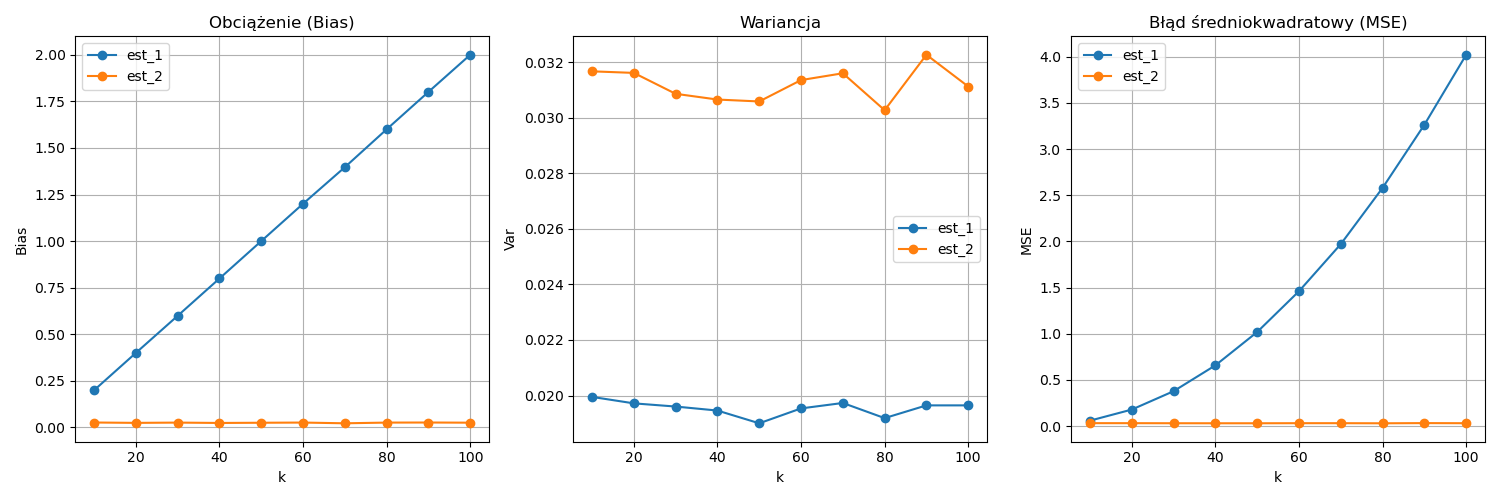
\includegraphics[width=1.1\textwidth]{../Zad3/plots/plot.png}
    \caption{Wykres kolejnych statystyk w zależności od parametru k.}
\end{figure}

\subsection{Dyskusja Wyników}

Eksperyment ten, polegający na wprowadzeniu pojedynczej obserwacji odstającej $k$ do próby z rozkładu $\mathcal{N}(0,1)$, w sposób jednoznaczny ilustruje pojęcie \textbf{odporności} estymatorów na obserwacje odstające.

\subsection*{Analiza Estymatora $\hat{\theta}_1$ (Średnia Arytmetyczna)}

Średnia arytmetyczna jest estymatorem znanym ze swojej wrażliwości na wartości ekstremalne. Przy stosunkowo niewielkiej próbie ($n=50$), wpływ pojedynczego punktu $k$ jest znaczący.

\begin{itemize}
    \item \textbf{Obciążenie:} Teoretyczne obciążenie średniej w tym eksperymencie wynosi:
    \[ \text{Bias}(\hat{\theta}_1) = E[\hat{\theta}_1] - \theta = E\left[ \frac{1}{n} \left(\sum_{i=1}^{n-1} X_i + k\right) \right]\]
    \[ \text{Bias}(\hat{\theta}_1) = \frac{1}{n} \left( \sum_{i=1}^{n-1} E[X_i] + k \right) = \frac{k}{n} \]
    Dla $n=50$, obciążenie wynosi $k/50$. Jest to funkcja \textbf{idealnie liniowo rosnąca} wraz ze wzrostem $k$, co powinno być widoczne na wykresach z symulacji.

    \item \textbf{Wariancja:} Co ciekawe, wariancja estymatora $\hat{\theta}_1$ nie jest zaburzona przez anomalię, ponieważ wariancja jest niezmiennicza względem przesunięcia:
    \[ \text{Var}(\hat{\theta}_1) = \text{Var}\left( \frac{1}{n} \left(\sum_{i=1}^{n-1} X_i + k\right) \right) = \frac{1}{n^2} \left( \sum_{i=1}^{n-1} \text{Var}(X_i) \right) \]
    \[ \text{Var}(\hat{\theta}_1) = \frac{1}{n^2} ( (n-1) \cdot 1 + 0 ) = \frac{n-1}{n^2} \]
    Dla $n=50$, wariancja jest stała i wynosi $49/2500 \approx 0.0196$, niezależnie od wartości $k$.

    \item \textbf{MSE:} Ponieważ $\text{MSE} = \text{Var} + \text{Bias}^2$:
    \[ \text{MSE}(\hat{\theta}_1) = \frac{n-1}{n^2} + \left(\frac{k}{n}\right)^2 = \frac{n-1 + k^2}{n^2} \]
    Wartość MSE jest zdominowana przez obciążenie i rośnie \textbf{kwadratowo} wraz ze wzrostem $k$.
\end{itemize}

\subsection*{Analiza Estymatora $\hat{\theta}_2$ (Mediana)}

Mediana jest klasycznym przykładem estymatora odpornego na obserwacje odstające.
\begin{itemize}
    \item Dopóki obserwacja odstająca $k$ jest wartością ekstremalną (co ma miejsce dla $k \ge 10$), będzie ona po prostu zajmować ostatnią pozycję $X_{(50)}$ i \textbf{nie będzie miała żadnego wpływu} na wyznaczenie wartości centralnych.
    \item W rezultacie, zarówno \textbf{obciążenie}, \textbf{wariancja}, jak i \textbf{MSE} estymatora $\hat{\theta}_2$ pozostają praktycznie \textbf{stałe} i niewrażliwe na wzrost $k$.
\end{itemize}

\subsection*{Wnioski}
Symulacje jednoznacznie potwierdzają teoretyczne przesłanki, że mediana jest estymatorem znacznie bardziej odpornym na ekstremalne obserwacje odstające niż średnia arytmetyczna.


\section{Zadanie 4}

\subsection{Opis eksperymentu}
W tym zadaniu w zależności od wartości parametrów: 

\begin{itemize}
    \item $\mu=0, \theta=1$
    \item $\mu=0, \theta=4$
    \item $\mu=4, \theta=1$
    \item $\mu=4, \theta=4$
\end{itemize}

esytmowano wariancję próby wielkości $n=50$ z rozkładu $N(\mu, \theta)$,

przy pomocy trzech esymatorów:

\begin{itemize}
    \item $\hat{\theta}_1 = S^{2} = \frac{1}{n-1}\sum_{i=1}^{n}(X_{i}-\bar{X})^{2}$
    \item $\hat{\theta}_2 = \frac{1}{n-1}\sum_{i=1}^{n}(X_{i} - median(X_{1}, \dots, X_{n}))^{2}$
    \item $\hat{\theta}_3 = median((X_1 - \bar{X})^{2}, \dots, (X_{n} -\bar{X})^2)$
\end{itemize}

Doświadczenie powtórzono $10{,}000$ razy. Porównano esymatory przy pomocy wyrkesów pudełkowych oraz
wyliczono wariancję, błąd średniokwadratowy oraz obciązenie każdego z esymatorów. 

\subsection{Wyniki}

\newcommand{\plotwithstatsIV}[2]{
    \subsection{$\mu=#1$, $\theta=#2$}
    \begin{figure}[H]
        \centering
        \includegraphics[width=0.9\textwidth]{../Zad4/plots/boxplot_mu_#1_theta_#2.png}
        \caption{Boxplot estymatorów dla $\mu=#1$, $\theta=#2$.}
    \end{figure}

    \begin{center}
    \csvreader[
        tabular=|l|c|c|c|c|,
        table head=\hline Estymator & Średnia & Wariancja & Bias & MSE \\ \hline,
        late after line=\\\hline,
        filter expr={true},  % brak filtrowania
        respect percent
    ]{../Zad4/plots/stats_mu_#1_theta_#2.csv}{Estimator=\est,Mean=\mean,Variance=\var,Bias=\bias,MSE=\mse}
    {\est & \pgfmathprintnumber{\mean} & \pgfmathprintnumber{\var} & \pgfmathprintnumber{\bias} & \pgfmathprintnumber{\mse} }
    \end{center}

    \newpage
}

\plotwithstatsIV{0}{1}
\plotwithstatsIV{0}{4}
\plotwithstatsIV{4}{1}
\plotwithstatsIV{4}{4}

\subsection{Dyskusja Wyników}

W tym zadaniu celem była estymacja parametru $\theta$, 
który w notacji rozkładu $\mathcal{N}(\mu, \theta)$ odpowiada \textbf{wariancji}.

\subsection*{Analiza Estymatora $\hat{\theta}_1 = S^2$}

Jest to klasyczny, \textbf{nieobciążony estymator wariancji} z próby.
\begin{itemize}
    \item \textbf{Obciążenie:} Zgodnie z rachunkami, które przeprowadziliśmy na wykładzie $E[S^2] = E[\hat{\theta}_1] = \sigma^2 = \theta$. 

    \item \textbf{MSE:} Ponieważ estymator jest nieobciążony, jego MSE jest równe jego wariancji: $\text{MSE}(\hat{\theta}_1) = \text{Var}(\hat{\theta}_1)$.

    Dokładnie to:
    \[
        \boxed{
            E[S^2] = \sigma^2, \quad \mathrm{Var}(S^2) = \frac{2\sigma^4}{n-1}
        }       
    \]
    \begin{itemize}
        \item Gdy $\theta = 1$ (wariancja populacji), $\text{MSE}(\hat{\theta}_1) = \frac{2 \cdot 1^2}{49} \approx 0.04$.
        \item Gdy $\theta = 4$ (wariancja populacji), $\text{MSE}(\hat{\theta}_1) = \frac{2 \cdot 4^2}{49} = \frac{32}{49} \approx 0.65$.
    \end{itemize}
    Wyniki eksperymentu zgadzają się z teoretycznymi obliczeniami.

\end{itemize}

\subsection*{Analiza Estymatora $\hat{\theta}_2$}

Estymator ten jest analogiczną konstrukcją do $S^2$, jednak zamiast optymalnego estymatora średniej $\bar{X}$, używa on estymatora odpornego -- \textbf{mediany} ($\hat{m} = \text{median}(X)$).
\begin{itemize}
    \item W rozkładzie normalnym $\hat{m}$ jest również nieobciążonym estymatorem $\mu$, jednak jest on \textbf{mniej efektywny} (ma większą wariancję) niż $\bar{X}$.
    \item Ponieważ do obliczenia $\hat{\theta}_2$ używamy "mniej dokładnego" oszacowania środka rozkładu, intuicyjnie spodziewamy się, że $\hat{\theta}_2$ będzie \textbf{nieco gorszym} estymatorem wariancji $\theta$ niż $\hat{\theta}_1$.
    \item Wyniki symulacji sugerują, że jest to estymator poprawny i bardzo zbliżony do $\hat{\theta}_1$, jednak różnica w biasie i MSE jest zauważalna.
\end{itemize}

\subsection*{Analiza Estymatora $\hat{\theta}_3$}

Estymator $\hat{\theta}_3 = \text{median}((X_i - \bar{X})^2)$ jest przykładem estymatora \textbf{obciążonego}.

\subsubsection*{Analiza asymptotyczna}

Aby formalnie wykazać obciążenie, zbadajmy granicę, do której zbiega estymator. Wraz ze wzrostem $n \to \infty$, średnia z próby $\bar{X}$ zbiega do $\mu$. Zatem $\hat{\theta}_3$ zbiega (według prawdopodobieństwa) do $m = \text{median}((X_i - \mu)^2)$.

Musimy wyznaczyć wartość tej mediany $m$.
\begin{itemize}
    \item Niech $X_i \sim \mathcal{N}(\mu, \theta)$.
    \item Standaryzujmy zmienną: $Z = (X_i - \mu) / \sqrt{\theta}$, gdzie $Z \sim \mathcal{N}(0, 1)$.
    \item Kwadrat tej zmiennej, $Z^2$, ma rozkład $\chi^2_1$ (Chi-kwadrat z 1 stopniem swobody).
\end{itemize}
Wartość $m$, do której zbiega estymator, to:
\[ m = \text{median}((X_i - \mu)^2) = \text{median}(\theta \cdot Z^2) = \theta \cdot \text{median}(\chi^2_1) \]

Mediana rozkładu $\chi^2_1$ to wartość $t$, dla której $P(Z^2 \le t) = 2\Phi(\sqrt{t}) - 1 = 0.5$. Jak wynika z obliczeń, $t = (\Phi^{-1}(0.75))^2 \approx (0.6745)^2 \approx \mathbf{0.4549}$.

\subsubsection*{Wnioski z symulacji}

Oznacza to, że estymator $\hat{\theta}_3$ nie zbiega do $\theta$, lecz do $\approx 0.4549 \cdot \theta$.
Fakt ten w pełni wyjaśnia wyniki obserwowane w symulacji:
\begin{itemize}
    \item Estymator wykazuje \textbf{znaczące obciążenie}, systematycznie zaniżając prawdziwą wariancję $\theta$ o około 55\%.
    \item Obserwacja z eksperymentu dla $\theta=4$ (gdzie wynik był $\approx 1.86$) jest bardzo bliska wartości teoretycznej, $4 \cdot 0.4549 \approx 1.82$.
    \item To duże obciążenie jest głównym składnikiem \textbf{wysokiego błędu średniokwadratowego (MSE)}, zgodnie ze wzorem $\text{MSE} = \text{Var} + \text{Bias}^2$.
\end{itemize}

\end{document}
